\documentclass{standalone}
\usepackage{amsmath,amssymb}
\usepackage{tikz}
\usepackage{circuitikz}
\usepackage{siunitx}
\begin{document}
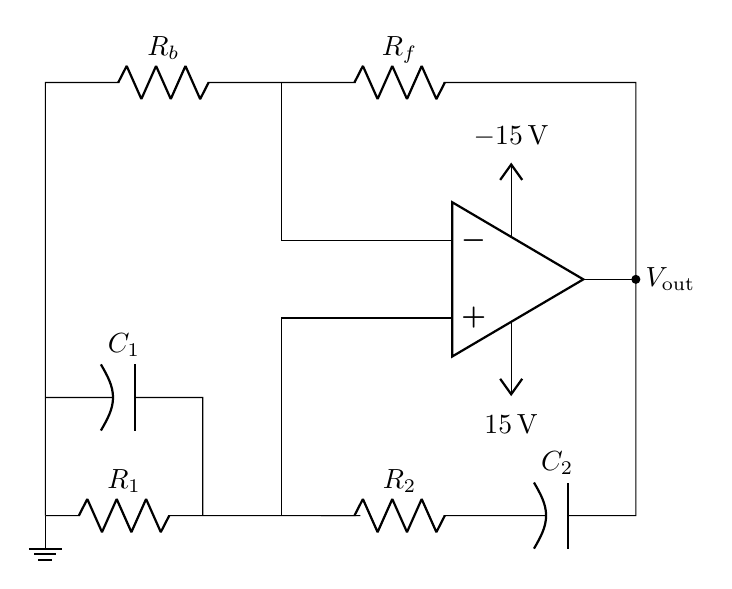
\begin{tikzpicture}
	\draw (0,0) node [op amp] (op) {};
	\draw (op.up) -- ++(0,0.5) node[vcc]{\SI{-15}{\volt}};
	\draw (op.down) -- ++(0,-0.5) node[vee]{\SI{15}{\volt}};
	\draw (op.+) -| (-3,-3);
	\draw (op.out) -- (1.5,0);
	\draw (1.5,0) -- (1.5, -3) to[pC, a=$ C_{2} $, invert] ++(-2,0)
	to[R, a=$ R_{2} $] ++(-2,0);
	\draw (-2, -3) -- ++(-2,0) to[R, a=$ R_{1} $] ++(-2,0) node[ground] {};
	\draw (-2, -3) ++(-2,0) -- ++(0, 1.5) to[pC, a=$ C_{1} $, invert] ++(-2,0);
	\draw (-6, -3) -- ++(0,5.5) to[R, l=$ R_{b} $] ++(3,0) to[R, l=$ R_{f} $] ++(3,0) -| (1.5,0);
	\draw (-3, 2.5) |- (op.-);
	\filldraw (1.5, 0) circle [radius=0.05] node[right] {$ V_{\rm out} $};
\end{tikzpicture}
\end{document}